% based on a template made by the university of cologne
% http://www.mi.uni-koeln.de/wp-MIEDV/wp-content/uploads/2016/07/LaTeX-Vorlage.zip - 2023-11-02
\documentclass[12pt,a4paper]{scrartcl}

\addtokomafont{sectioning}{\rmfamily}
\usepackage[ngerman]{babel}% deutsches Sprachpaket wird geladen
\usepackage[T1]{fontenc} % westeuropäische Codierung wird verlangt
\usepackage[utf8]{inputenc}% Umlaute werden erlaubt
\usepackage[usenames]{color} % Erlaubt die Benutzung der namen im Farbpaket und deren Änderung
\usepackage{amsmath} % Erweiterung für den Mathe-Satz
\usepackage{amssymb} % alle Zeichen aus msam und msmb werden dargestellt
\usepackage{graphicx} % Graphiken und Bilder können eingebunden werden
%\usepackage{multirow} % erlaubt in einer Spalte einer Tabelle die Felder in mehreren Zeilen zusammenzufassen
\usepackage{enumerate} % erlaubt Nummerierungen
\usepackage{xurl} % Dient zur Auszeichnung von URLs; setzt die Adresse in Schreibmaschinenschrift.
\usepackage[center]{caption}  % Bildunterschrift wird zentriert
%\usepackage{subfigure} % mehrere Bilder können in einer fugure-Umgebung verwendet werden
%\usepackage{longtable} % Diese Umgebung ist ähnlich definiert wie die tabular-Umgebung, erlaubt jedoch mehrseitige Tabellen.
%\usepackage{paralist} % Modifikation der bereits bestehenden Listenumgebungen
\usepackage{lmodern}% Für die Schrift
\usepackage[hidelinks]{hyperref} % Links und Verweise werden innerhalb von PDF Dokumenten erzeugt
%\usepackage{wrapfig} % Das Paket ermöglicht es von Schrift umflossene Bilder und Tabellen einzufügen.
\usepackage{latexsym} % LaTeX-Symbole werden geladen
\usepackage{tikz} % Erlaubt es mit tikz zu zeichnen
\usepackage{tabularx} % Erlaubt Tabellen
\usepackage{algorithm} % Erlaubt Pseudocode
\usepackage{color} % Farbpaket wird geladen
%\usepackage{stmaryrd} % St Mary Road Symbole werden geladen
\usepackage{physics}

\numberwithin{equation}{section} % Nummerierungen der Gleichungen, die durch equation erstellt werden, sind gebunden an die section
\newcommand{\HRule}{\rule{\linewidth}{0.7mm}}

\hypersetup{
  pdftitle={B 2.5},
  pdfcreator={LaTeX via pandoc}
}

\setcounter{secnumdepth}{6}
\setcounter{tocdepth}{6}

\begin{document}
\begin{titlepage}
	\pagestyle{empty}

	\begin{center}

	\textsc{\LARGE Universität zu Köln }\\ [0.4cm]
	\textsc{Mathematisch-Naturwissenschaftliche Fakultät} \\[1.5cm]

	
\includegraphics[width=0.45\textwidth]{../media/uni.jpg}\\[1.5cm]  % Uni-Logo wird geladen

	\textsc{\Large Praktikum~B}\\[2mm]
	\textsc{}\\[10mm]
	\HRule \\[0.4cm]

		{	\Huge \bfseries B 2.5}\\[0.4cm]
			{	\huge \bfseries Rastertunnelmikroskopie}\\[0.3cm]
	
	\HRule \\[3cm]

		\textsc{\Large Catherine Tran } \\[3pt]
		\textsc{\Large Carlo Kleefisch } \\[3pt]
		\textsc{\Large Oliver Filla } \\[3pt]
		
	\end{center}
\end{titlepage}

\newpage
\tableofcontents
\newpage

\hypertarget{motivation}{%
\section{Motivation}\label{motivation}}

Mit einem Rastertunnelmikroskop\footnote{engl. Scanning Tunneling  Microscope (STM)} (STM) können Oberflächenstrukturen in der Größe von Atomen gemessen werden, wenn die Oberfläche elektrischen Strom leitet.

In diesem Experiment werden zwei verschiedene Proben, eine aus Gold und eine aus Graphit, vermessen. Als die Graphitprobe wird hochorientiertes pyrolytisches Graphit (HOPG) verwendet, was eine besonders stabile Struktur aufweist.

\clearpage
\hypertarget{theoretische-grundlagen}{%
\section{Theoretische Grundlagen}\label{theoretische-grundlagen}}
\hypertarget{tunnelspektroskopie}{%
\subsection{Tunnelspektroskopie}\label{tunnelspektroskopie}}
Mit dem Rastertunnelmikroskop (STM) lässt sich die \textit{atomare Topographie} einer Probe darstellen. Hierbei werden keine Atome aufgelöst, stattdessen wird eine Ladungsdichtedifferenz zwischen Spitze und Probe abgebildet.

Ein Atom erscheint größer, wenn nur eine geringe Austrittsarbeit notwendig ist, um ein Elektron
über die Fermikante zu bringen. Ist die notwendige Austrittsarbeit höher, wird der Atom kleiner dargestellt.

Neben der Auflösung einer Oberfläche lässt sich durch gezielte Variation von bestimmten Parametern \textit{Tunnelspektroskopie} betreiben. Damit lassen sich weitere Eigenschaften der Probe zu messen.

Dabei werden zwei Messmodi verwendet. Zum einen gibt es den den \textit{Konstant--Höhen--Modus}, bei dem die Tunnelspitze parallel zur Oberfläche der Probe bewegt wird. Existiert Unebenheit, dann variiert das Signal vom Tunnelstrom stark und man kann daraus topographische Rückschlüsse ziehen. In diesem Modus lassen sich mithilfe von $I(V)$--\textit{Spektroskopie} Informationen über die Zustandsdichte herausfinden.

Bei der zweite Methode wird die Tunnelspannung konstant gehalten und der Abstand zwischen Spitze und Probe so eingestellt, bis man einen nahezu konstanten Stromsignal bekommt. Dieses kann durch gute Regelung des Abstandes zu erreicht werden. Auch hier erhält man Informationen über die Oberfläche der Probe. Die Methode wird \textit{Konstant--Strom--Modus} genannt.

Fixiert man einen Punkt und zieht die Spitze dann hoch, lässt sich aus dem Tunnelstrom die Austrittsarbeit bestimmen. Daher nennt man diese Methode \textit{$I(z)$--Spektroskopie}. Da der Tunnelstrom $I$ exponenziell von der Höhe $z$ abhängig ist \eqref{eq:Tunnelstrom}, erhält man eine gute Auflösung.\footnote{vgl. \ref{auflösung}: \nameref{auflösung}}

\hypertarget{tunneleffekt}{%
\subsubsection{Tunneleffekt}\label{tunneleffekt}}
Quantenmechanische Teilchen können Potentialbarrieren auch dann überwinden, wenn ihre Energie eigentlich zu niedrig ist. Man spricht davon, dass sie durch die Barriere hindurchtunneln. Abbildung \ref{abb:tunneleffekt} stellt dies qualitativ für eine Wellenfunktion mit einer Energie $E$ und ein Kastenpotential der Höhe $V>E$ dar.

\begin{figure}[ht]
	\centering
	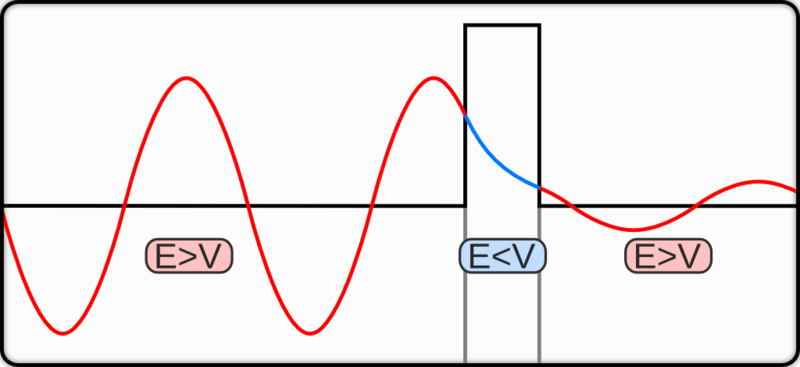
\includegraphics[width=0.7\textwidth]{../media/B2.5/800px-TunnelEffektKling1.png}
	\caption{Qualitativer Verlauf der Wellenfunktion, \\die Welle trifft von links auf die Potentialbarriere
		\cite{WikipediaTunneleffekt}\\}
	\label{abb:tunneleffekt}
\end{figure}

Die tatsächliche Potentialbarriere kann analog zur Gamow--Näherung als einzelnes kastenförmiges Potential $V(z)$ angenommen werden. Die Potentialbarriere beginne an der Position $0$ bei der Probe und ende an der Position $z_0$ an der Messspitze des STMs.

\begin{eqnarray}
	V(z) &=&
	\begin{cases}
		V_0 &: z \in [0, z_0] \\
		0 &: z \notin [0, z_0]
	\end{cases}
\end{eqnarray}
Aus der allgemeinen Schrödingergleichung \eqref{eq:SGL allg} lässt sich die eindimensionale stationäre Form \eqref{eq:SGL} herleiten, wofür neben dem Potential $V(z)$ die Elektronenmasse $m_e$ benötigt wird.

\begin{eqnarray}
	i\hbar \ket{\dot{\Psi}} &=& \hat H\ket{\Psi} \label{eq:SGL allg} \\
	E_n\Psi_n(z) &=&
		\left(
			-\frac{\hbar^2}{2m_e} \frac{\partial^2}{\partial z^2} + V(z)
		\right)\Psi_n(z)
		\label{eq:SGL}
\end{eqnarray}
Die Lösung von \eqref{eq:SGL} liefert die Tunnelwahrscheinlichkeit $P(z_0)$, mit der das Teilchen die Barriere durchtunnelt. Der relevante Parameter $\kappa$ ist abhängig von der Elektronenmasse $m_e$, der Höhe der Potentialbarriere $V_0$ und der Energie $E$ des tunnelnden Elektrons. $\hbar$ ist die reduzierte Planck--Konstante.

\begin{eqnarray}
	P(z_0) &\propto& |\Psi(0)|^2 \cdot \mathrm e^{-2\kappa z_0} \\
	\kappa &=& \frac{\sqrt{2m_e(V_0 - E)}}{\hbar} \label{eq:Tunnelwkt Kappa}
\end{eqnarray}
Diese Wahrscheinlichkeit ist exponentiell von der Breite des Potentials $z_0$ abhängig. Zudem ist sie von der Wahrscheinlichkeit für den Aufenthalt eines Teilchens am Beginn der Probe abhängig, die durch die quadrierte Wellenfunktion $|\Psi(0)|^2$. Dies ist in Abbildung \ref{abb:tunneleffekt} im Bereich der Potentialbarriere ersichtlich.

Diese Wahrscheinlichkeit hängt davon ab, wie wahrscheinlich ein Elektron aus der Probe austritt. Dazu ist die Austrittsenergie $\phi$ essentiell. Dafür wiederum ist die Besetzung der Energieniveaus relevant, die von der Temperatur und der Fermi--Energie abhängt. Die Beschreibung erfolgt durch die Zustandsdichte.

Für das STM ist jedoch nicht der Einzelfall interessant, sondern die Rate, mit der Elektronen aus der Probe austreten und tunneln. Dies kann durch den \emph{Tunnelstrom} $I$ beschrieben werden.

Der Tunnelstrom ist proportional zur Tunnelwahrscheinlichkeit $P(z_0)$, ebenso zu der Anzahl der Elektronen, die in einer gewissen Zeit aus dem Material austreten. Dadurch ist der Tunnelstrom exponentiell von der Breite $z_0$ der Potentialbarriere abhängig.

\begin{eqnarray}
	I(z_0) &\propto& \mathrm e^{-2\kappa z_0} \label{eq:Tunnelstrom}
\end{eqnarray}
Durch die exponentielle Abhängigkeit des Tunnelstroms $I$ von dem Abstand $z_0$ ist ein STM sehr sensibel gegen Höhenunterschieden. Schon ein Höhenunterschied von $1\,\mathrm{\mathring{A}}$ macht einen Faktor von näherungsweise $8$ im Tunnelstrom aus. \cite{Anleitung} Dadurch können Atomstrukturen an der Oberfläche gemessen werden.

\hypertarget{piezoelektrischer-effekt-und-anwendung}{%
\subsubsection{piezoelektrischer Effekt und Anwendung}\label{piezoelektrischer-effekt-und-anwendung}}

Der piezoelektrische Effekt bezeichnet die Erzeugung elektrischer Spannungen an bestimmten Kristallen, den Piezokristallen, bei deren Deformation. Dies funktioniert auch umgekehrt: Durch Anlegen einer Spannung verformt sich ein Piezokristall. Dies nennt man \emph{inversen Piezoeffekt}.

Der inverse Piezoeffekt wird zur Bewegung der Messspitze verwendet. Diese ist an einer Platform befestigt, die auf drei Piezoröhrchen steht. Durch Anlegen von Spannung an diesen Röhrchen verformen diese sich. Wird die Spannung langsam angelegt und plötzlich entfernt, so geschieht diese Verformung erst langsam, dann sprunghaft.

Wird die Spannung auf diese Weise bei allen drei Piezoröhrchen variiert, so wird die Position der Messspitze verändert. Hierbei gibt es die zwei Variationen: Entweder kann die Position auf der Probenoberfläche verändert werden, beispielsweise kann nach rechts ``gewandert'' werden.

Alternativ kann die Messspitze rotiert werden, ohne die Position auf der Probenoberfläche zu verändern. Dies kann dazu genutzt werden, um die Höhe der Messspitze zu steuern.

\hypertarget{auflösung}{
\subsubsection{Auflösung des STM}\label{auflösung}}
Das Rastertunnelmikroskop besitzt eine sehr hohe vertikale sowie laterale Auflösung, was die atomare Abbildung von Proben erstmals möglich machte.

Die vertikale Auflösung ist sehr hoch. Dies kommt zustande, da der Tunnelstrom $I$ exponentiell vom Abstand $z$ abhängig ist, wie es in Gleichung \eqref{eq:Tunnelstrom} beschrieben wird.

Daher sorgt eine kleine Änderung in der Tunnelbreite $z$ für große Änderungen im Tunnelstrom $I$. Hat die Probe also auch nur kleine Höhenunterschiede, sind diese im resultierenden Bild deutlich sichtbar.

Auch die horizontale Auflösung basiert auf der Proportionalität des Tunnelstroms zur Tunnelbreite. Auf der Spitze des STM gibt es immer ein Atom, dass der Probe am nächsten liegt, welches den Elektronen die kleinste Tunnelbreite $z_0$ zum tunneln liefert. Alle weiteren Atome auf der Spitze machen es den Elektronen ebenfalls möglich zu tunneln, allerdings mit einer höheren Tunnelbreite $z_i > z_0$.

Aufgrund von \eqref{eq:Tunnelstrom} folgt, dass der Beitrag des nächsten Atoms $I_0$ zum Gesamttunnelstrom deutlich größer ist als der Beitrag aller anderen Atome auf der Spitze $I_i$. Der Tunnelstrom $I$, wird also vom Atom, dass der Probe am nächsten ist, dominiert, wodurch eine atomare Abtastung in guter Näherung gegeben ist.

\hypertarget{kristallstruktur}{%
\subsection{Kristallstruktur}\label{kristallstruktur}}
Die atomare Struktur eines Festkörpers wird durch eine Basis und ein Gitter beschrieben. Die Basis besteht aus Atomen oder Molekülen, die an jedem Gitterpunkt eines Kristallgitters angeheftet ist.

Unter dem Begriff \textit{Kristallgitter} versteht man eine räumlich regelmäßige Anordnung von Punkten. Allerdings sind nur die Bravais--Gitter zur Beschreibung von Kristallen sinnvoll.

Ein \textit{Bravais--Gitter} besitzt eine bis ins Unendliche ausgedehnte Anordnung von Gitterpunkten, die von jedem Punkt aus gleich aussieht. Alternativ wird es durch die Translationen $\vec{R} = n_1\vec{a}_1 + n_2\vec{a}_2 + n_3\vec{a}_3$ definiert. Es gibt $14$ verschiedene Bravais--Gitter.

Erfüllt eine Zelle den Raum ohne Lücke und ohne Überlapp, wenn diese Zelle mit allen $\vec{R}$ verschoben wird, so heißt sie \textit{primitive Einheitszelle}. Sie ist nicht eindeutig definiert und enthält genau einen Gitterspunkt. Eine mögliche primitive Einheitzelle ist in Abbildung \ref{abb:bravais} blau dargestellt, wobei die grünen Kugeln Gitterpunkte darstellen.

Eine \textit{konventionelle Einheitszelle} spiegelt die Symmetrie des Gitters dar und kann mehrere Gitterpunkte beinhalten. Sie ist in Abbildung \ref{abb:bravais} grün dargestellt, in diesem Beispiel enthält sie $2$ Gitterpunkte.

\begin{figure}[ht]
	\centering
	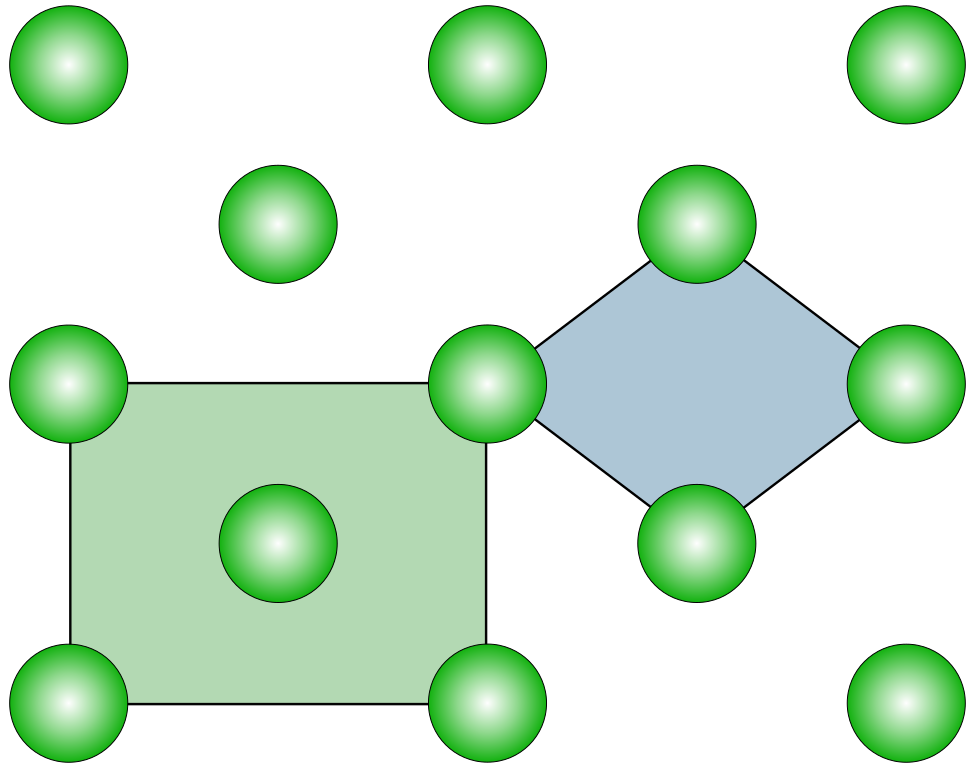
\includegraphics[width=0.5\textwidth]{../media/B2.5/975px-Rectangular_unit_cells_centered.svg.png}
	\caption{Bravais--Gitter mit konventioneller bzw. primitiver Einheitszelle \cite{WikipediaBravaisgitter}}
	\label{abb:bravais}
\end{figure}

\hypertarget{graphitstruktur}{%
\subsubsection{Graphit}\label{graphitstruktur}}
Graphit besteht aus Graphenschichten in der hexagonalen Struktur mit der Stapelfolge $ABAB$. In jeder Schicht sind die Kohlenstoffatome in der Honigwabenstruktur mit einem Abstand von $142\mathrm{\,pm}$ angeordnet. Der Abstand zwischen zwei Lagen beträgt $335\mathrm{\,pm}$, zwischen ihnen herrschen schwache Van--der--Waals--Kräfte.

Im dem Versuch wird hochorientiertes pyrolytisches Graphit (HOPG) verwendet, das einen besonders hohen Grad an Ordnung hat und daher einfach präperiert werden kann.

\hypertarget{goldstruktur}{%
\subsubsection{Gold}\label{goldstruktur}}
Gold kristallisiert in einer kubisch--flächenzentrierten Struktur mit einer Kantenlänge von $407\mathrm{\,pm}$, dargestellt in Abbildung \ref{abb:fcc}. Die primitive Einheitszelle ist rhomboedrisch mit einer einatomigen Basis.

Das in diesem Versuch verwendete Gold ist entweder ein Goldblech oder Gold auf Glimmer. Der verwendete Glimmer besteht aus Aluminiumsilikatschichten, die einzelne Schichten sind schwach durch Kaliumionen gebunden. Dadurch kann man das Material einfach spalten und eine glatte Oberfläche erhalten.

Das Goldblech ist ein Polykristall aus $99.9\,\%$ Gold. Die Textur ist weniger ausgeprägt als Gold auf Glimmer. Beide Probe müssen vor dem Experimentieren thermisch gereinigt und geglättet werden.


\begin{figure}[ht]
	\begin{minipage}[b]{0.5\textwidth}
		\centering
		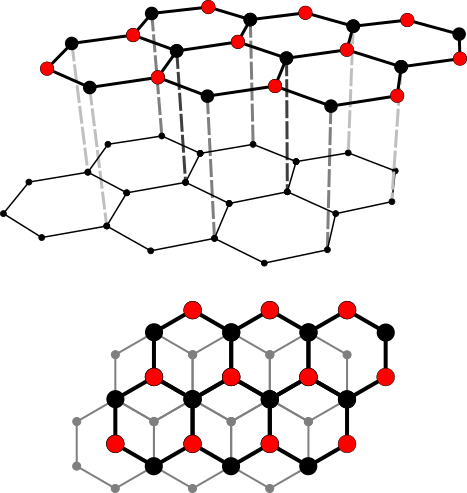
\includegraphics[width=0.75\textwidth]{../media/B2.5/Graphit_gitter4.png}
		\caption{Gitterstruktur Graphit \cite{WikipediaGraphit}}
	\end{minipage}
	\begin{minipage}[b]{0.5\textwidth}
		\centering
		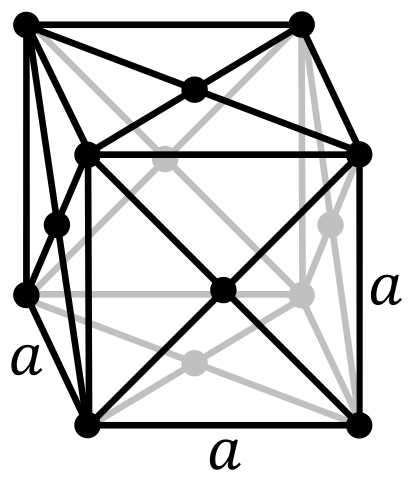
\includegraphics[width=0.6\textwidth]{../media/B2.5/412px-Cubic-face-centered.svg.png}
		\caption{fcc--Gitter \cite{WikipediaFcc}}
		\label{abb:fcc}
	\end{minipage}
\end{figure}

\hypertarget{defekte}{
\subsection{Kristall- und Oberflächendefekte}\label{defekte}}
Im thermodynamischen Gleichgewicht bei endlichen Temperaturen existieren keine defektfreien Kristalle. So werden auch die Proben in diesem Versuch Defekte aufweisen, die mittels des STM sichtbar gemacht werden können. Dabei lassen sie sich aufgrund ihrer Dimensionalität grob in drei Kategorien einordnen, namentlich Punktdefekte, Liniendefekte und Flächendefekte. Zwei Arten von Liniendefekten werden im Folgenden erläutert.

\hypertarget{korngrenzen}{
\subsubsection{Korngrenzen}\label{korngrenzen}}
Korngrenzen treten auf, wenn mehrere einkristalline Bereiche im Kristall mit unterschiedlicher Orientierung aufeinandertreffen. Sie gehören zu der Kategorie der Flächendefekte und sind in Abbildung \ref{abb:Korngrenzen} dargestellt. \cite{Gross} % [S. 43]

\begin{figure}[ht]
	\centering
	\begin{minipage}[t]{0.3\textwidth}
		\centering
		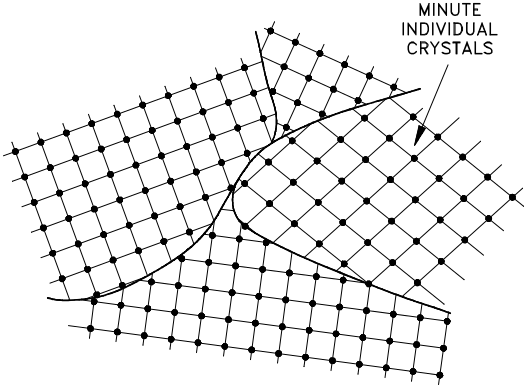
\includegraphics[width=\textwidth]{../media/B2.5/Korngrenzen.png}
		\caption{Korngrenzen \cite{USDoE}}
		\label{abb:Korngrenzen}
	\end{minipage}
	\begin{minipage}[t]{0.3\textwidth}
		\centering
		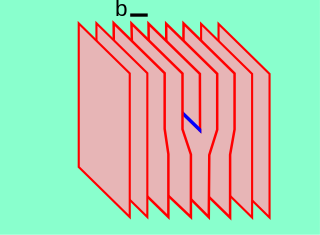
\includegraphics[width=\textwidth]{../media/B2.5/320px-Dislocation_edge_d2.svg.png}
		\caption{Stufenversetzung \cite{WikipediaStufe}}
		\label{abb:Stufenversetzung}
	\end{minipage}
	\begin{minipage}[t]{0.3\textwidth}
		\centering
		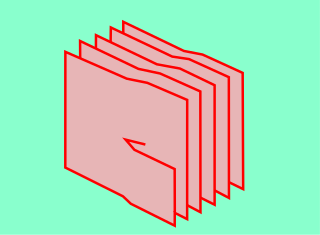
\includegraphics[width=\textwidth]{../media/B2.5/320px-Dislocation_screw_e.svg.png}
		\caption{Schraubenversetzung \cite{WikipediaSchraube}}
		\label{abb:Schraubenversetzung}
	\end{minipage}
\end{figure}

\hypertarget{versetzungen}{
\subsubsection{Versetzungen}\label{versetzungen}}
Versetzungen gehören zu den Liniendefekten und können in unterschiedlichen Formen auftreten. Die zwei wichtigsten sind Stufen- und Schraubenversetzungen.

Die Entstehung von Stufenversetzungen lässt sich mit der Vorstellung verbildlichen, dass  ein Kristall entlang einer Ebene $ABCD$ horizontal von der Linie $AB$ bis zur Linie $CD$ aufgeschnitten wird. Der Teil des Kristalls oberhalb der Schnittfläche wird nun um eine Gitterkonstante $a$ nach rechts in Richtung $BC$ verschoben, danach wird der Kristall wieder zusammengefügt. Nachdem ein Spannungsausgleich stattgefunden hat, ist der Teil des Kristalls unterhalb der Schnittfläche gedehnt. Die Versetzungslinie ist entlang $CD$ zu sehen, in Abbildung \ref{abb:Stufenversetzung} blau dargestellt.

Bei der Schraubenversetzung wird der Kristall zunächst erneut wie oben beschrieben aufgeschnitten. Dann wird allerdings ein Teil des Kristalls oberhalb des Schnittes nach hinten in Richtung der Linie $CD$ verschoben. Dies ist in Abbildung \ref{abb:Schraubenversetzung} zu sehen.

Versetzungen lassen sich auch charakterisieren, indem gedanklich einmal um den Versetzungskern herumgelaufen wird. Herumlaufen meint dabei, dass gleich viele Schritte in jede Richtung gemacht werden. Besitzt ein Kristall keine Versetzungen, bildet dieser Weg einen Kreis, man kommt wieder am Ausgangspunkt an. Sind allerdings Versetzungen vorhanden, ist der Weg nicht geschlossen. Der fehlende Weg wird Burgers--Vektor $\vec{b}$ genannt.

Bei Stufenversetzungen steht $\vec{b}$ senkrecht auf der Versetzungslinie, bei Schraubenversetzungen parallel. \cite{Gross} % [S. 42f]
Versetzungen können entlang des Burgers--Vektors $\vec{b}$ verschoben werden. Dies führt zu plastischer Verformung des Materials.

Die Ebenen, auf denen Versetzungen wandern, werden Gleitebenen genannt. Sie sind dadurch ausgezeichnet, dass die benötigte kritische Schubspannung auf diesen Ebenen minimal ist.

\clearpage
\hypertarget{durchfuxfchrung}{%
\section{Durchführung}\label{durchfuxfchrung}}

\hypertarget{gold}{%
\subsection{Gold}\label{gold}}

\hypertarget{strukturmessung}{%
\subsubsection{Strukturmessung}\label{strukturmessung}}

Zunächst wird die grobe Struktur von Gold gemessen, dabei wird eine Stufenkante gesucht. Dies erweist sich als schwierig, da die Probe kontaminiert ist. Es entstehen keine scharfen Bilder, allerdings gibt es eine Stelle mit mehreren scharfen Kanten. Diese sehen jedoch nicht nach Gold aus, vermutlich wurde ein Fremdkörper vermessen.

Die Probe ist zerkratzt, dies ist mit dem bloßen Auge sichtbar. Andere Kontaminationen, u.\,a. biologischer Natur, werden explizit nicht ausgeschlossen. Auf das Reinigen und Präperieren der Probe wurde verzichtet, da schon weitaus aufwendigere und invasivere Methoden versucht wurden als die, welche uns in diesem Versuch zur Verfügung stehen würden.

\hypertarget{austrittsarbeit}{%
\subsubsection{Austrittsarbeit}\label{austrittsarbeit}}

Zur Messung der Austrittsarbeit wird die Messspitze an der selben Position in der Höhe verändert, dabei wird der Tunnelstrom $I(z)$ gemessen. Im ersten Teil wird sie um $3\,\mathrm{\mathring{A}}$ abgesenkt und wieder angehoben, im zweiten Teil wird die Messspitze stattdessen um $3\,\mathrm{\mathring{A}}$ angehoben und wieder abgesenkt.

\hypertarget{graphit}{%
\subsection{Graphit}\label{graphit}}

Wie bei der Goldprobe wird zunächst ein grobes Bild der Struktur gemessen. Dabei soll eine glatte Stelle gefunden werden, an der eine Detailaufnahme der Atomstruktur aufgenommen wird.

Wie auch die Goldprobe ist auch diese Probe zerkratzt, was wieder mit bloßem Auge zu erkennen ist, und auch hier wurde auf Reinigung und Präperation verzichtet.

\clearpage
\hypertarget{auswertung}{%
\section{Auswertung}\label{auswertung}}
Die Bilder der Messungen wurden mit der Software \href{http://gwyddion.net}{Gwyddion} \cite{Gwyddion} erstellt und ausgewertet.

\hypertarget{gold-1}{%
\subsection{Gold}\label{gold-1}}

Die im Versuch aufgenommenen Bilder von Gold sind alle sehr verschieden. Auf einigen ist das Rauschen zu groß und es sind amorphe Region zu sehen, deshalb werden sie nicht im Protokoll weiter diskutiert. Daher wurden uns vonseiten der Versuchsbetreung zusätzliche Daten zur Auswertung bereitgestellt. \cite{Grover}

\hypertarget{eigene-messung}{%
\subsubsection{eigene Messung}\label{eigene-messung}}
In Abbildung \ref{abb:Gold gross} kann man mögliche Stufenkanten sehen. Das darunterliegende Gebiet ist nicht eindeutig zu identifizieren. Vermutlich erstrecken sich viele Stufenkanten über diesem Bild, was aber wegen Rauschen im Messsignal unklar ist.

Die gesamte Struktur sieht nicht nach einem Einkristall aus. Dies legt die Vermutung nahe, dass Fremdkörper auf der Probe sind.

\begin{figure}[ht]
	\centering
	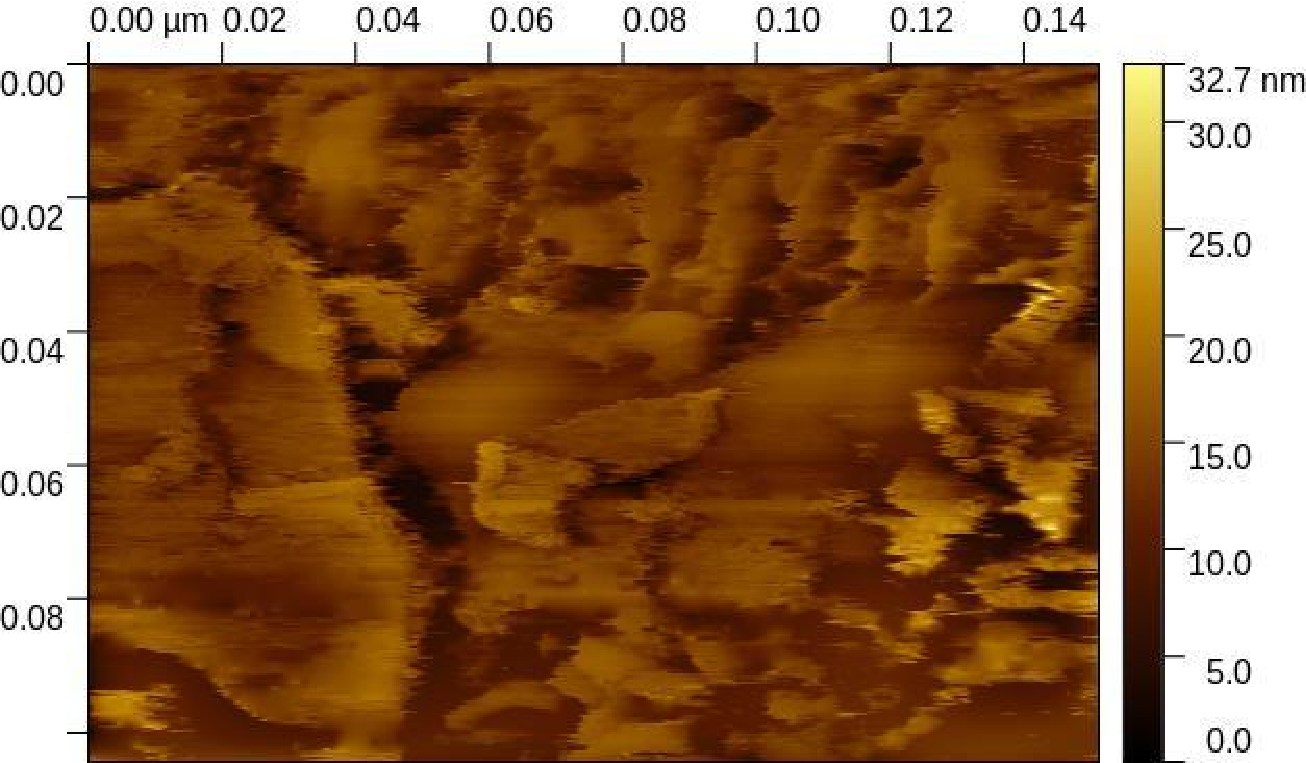
\includegraphics[width=0.7\textwidth]{../media/B2.5/Gold_gross.pdf}
	\caption{Großaufnahme der Goldoberfläche, \\
		Bias-Spannung $468\mathrm{\,mV}$, Strom $4.4 \mathrm{\,nA}$}
	\label{abb:Gold gross}
\end{figure}
	
\begin{figure}[ht]
	\centering
	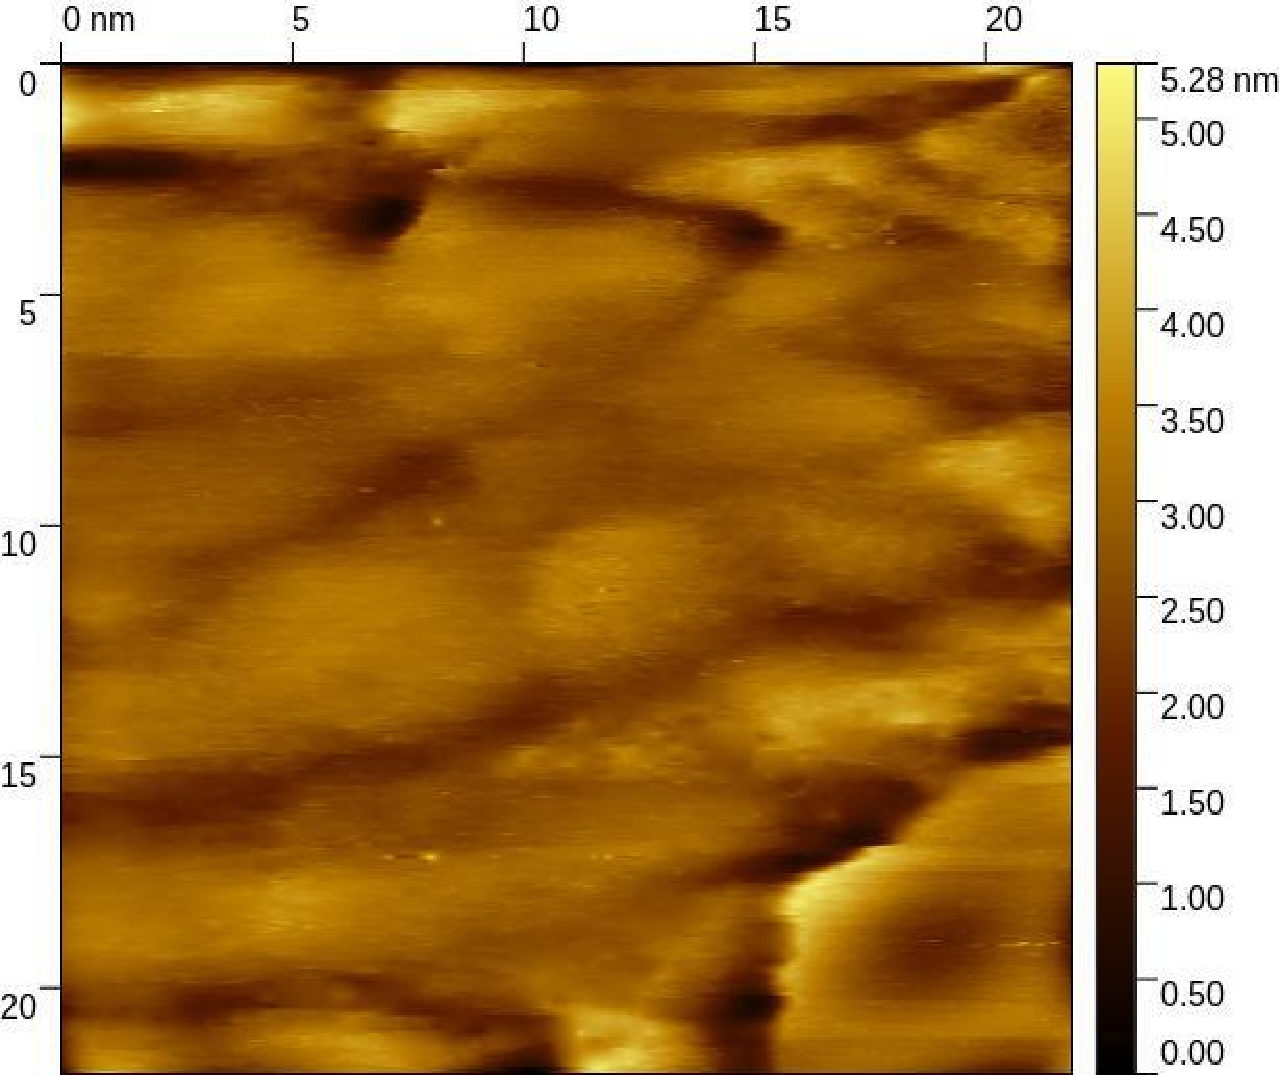
\includegraphics[width=0.7\textwidth]{../media/B2.5/Gold_Stufenkante.pdf}
	\caption{Nahaufname einer anderen Region, \\
		Bias-Spannung $468\mathrm{\,mV}$, Strom $4.7 \mathrm{\,nA}$}
	\label{abb:Gold stufe}
\end{figure}

Bei Abbildung \ref{abb:Gold stufe} erkennt man eine mögliche Terrassenstruktur, die von links nach rechts verlaufen. Auch hier leiden die Bilddetails unter der schlechten Qualität, scharfe Kanten sind nicht zu erkennen. Möglicherweise gibt es auch hier Fremdstoffe, die z.B. die Leitfähigkeit oder die Tunnelwahrscheinlichkeit beeinflussen.

Biologisches Material wie Fettspuren könnten diese Bilder erklären.

\newpage
\hypertarget{bereitgestelltes-material}{%
\subsubsection{bereitgestelltes
Material}\label{bereitgestelltes-material}}

In Abbildung \ref{abb:Gold Stufenkante} kann man eine Stufenkante in der Höhe von $1.03\mathrm{\,nm}$ in der oberen rechten Bildhälfte erkennen. Die Oberfläche scheint sehr glatt zu sein, wobei auch hier ein Rauschen im Bild auftritt.

\begin{figure}[ht]
	\centering
	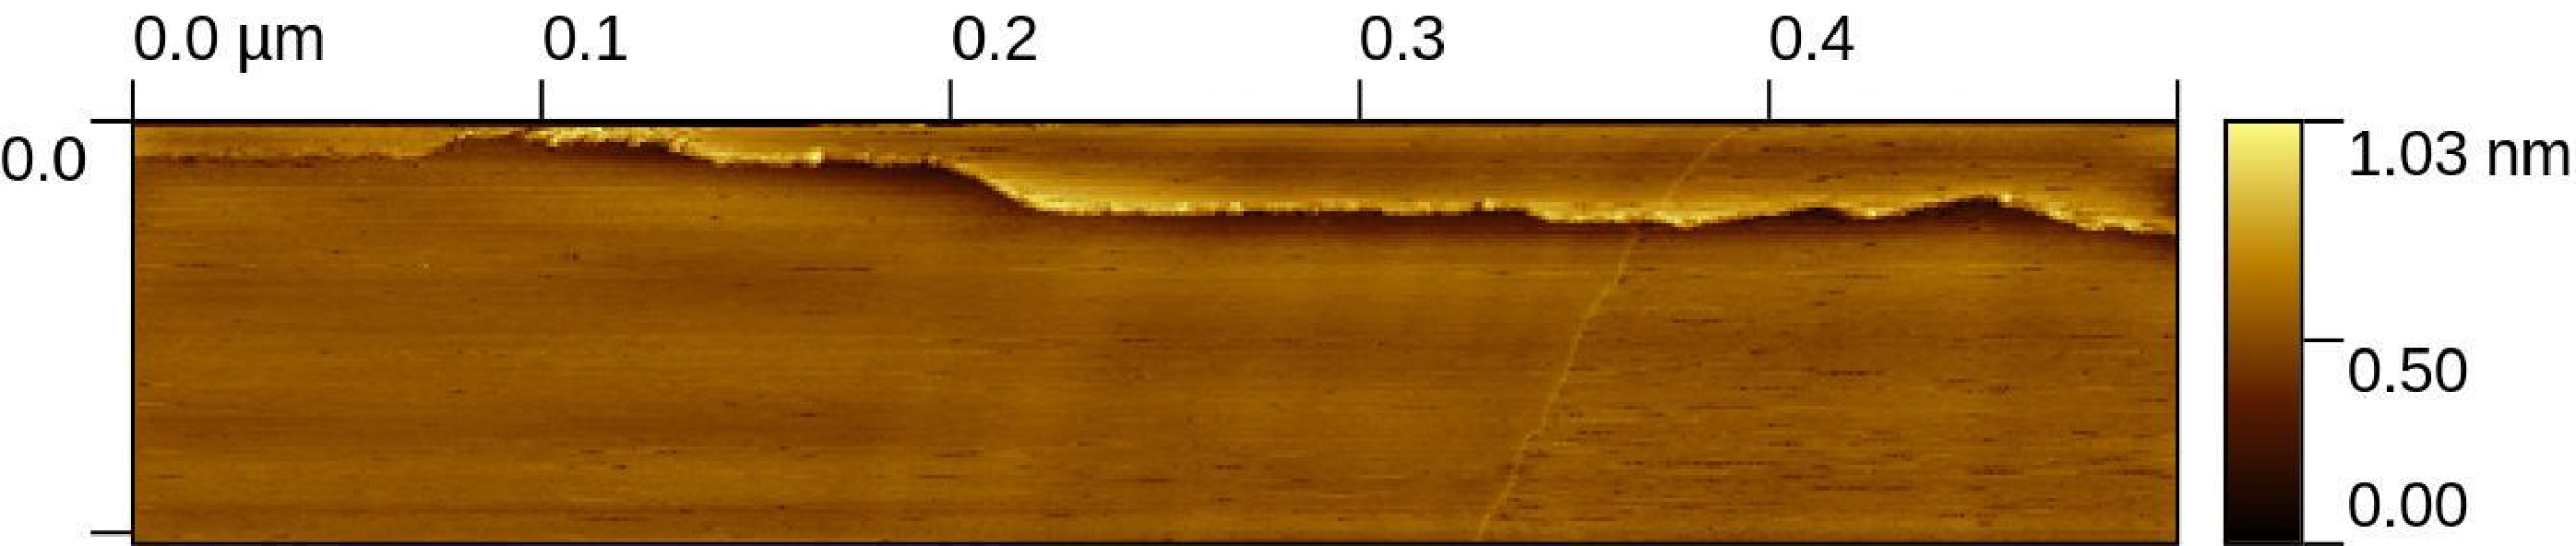
\includegraphics[width=0.7\textwidth]{../media/B2.5/Stufenkante.pdf}
	\caption{Großaufnahme einer Stufenkante, Quelle: \cite{Grover}, \\
			Bias-Spannung $499.94 \mathrm{\,mV}$, Strom $0.75 \mathrm{\,nA}$}
	\label{abb:Gold Stufenkante}
\end{figure}

Die Stufenkante entsteht bei der Abkühlung nach dem Ausglühen der Probe, d.h. durch die thermische Spannung. Gold besitzt eine $\mathrm{fcc}$--Gitterstruktur, so treten die Stufenversetzungen in den $\expval{1\,1\,1}$--Ebenen auf. Diese sind zugleich die dichtgepackten Ebenen. Die Stufenkante verläuft in die selbe Richtung wie der Burgersvektor, nämlich in die $\expval{1\,1\,0}$--Richtungen.

In Abbildung \ref{abb:Gold terassen} sind Terrassen abgebildet, die von Stufenkanten getrennt sind. Die Stufen verlaufen von unten rechts nach oben links und die Breite der einzelnen Stufen scheinen relativ gleichmäßig zu sein.

\begin{figure}[ht]
	\centering
	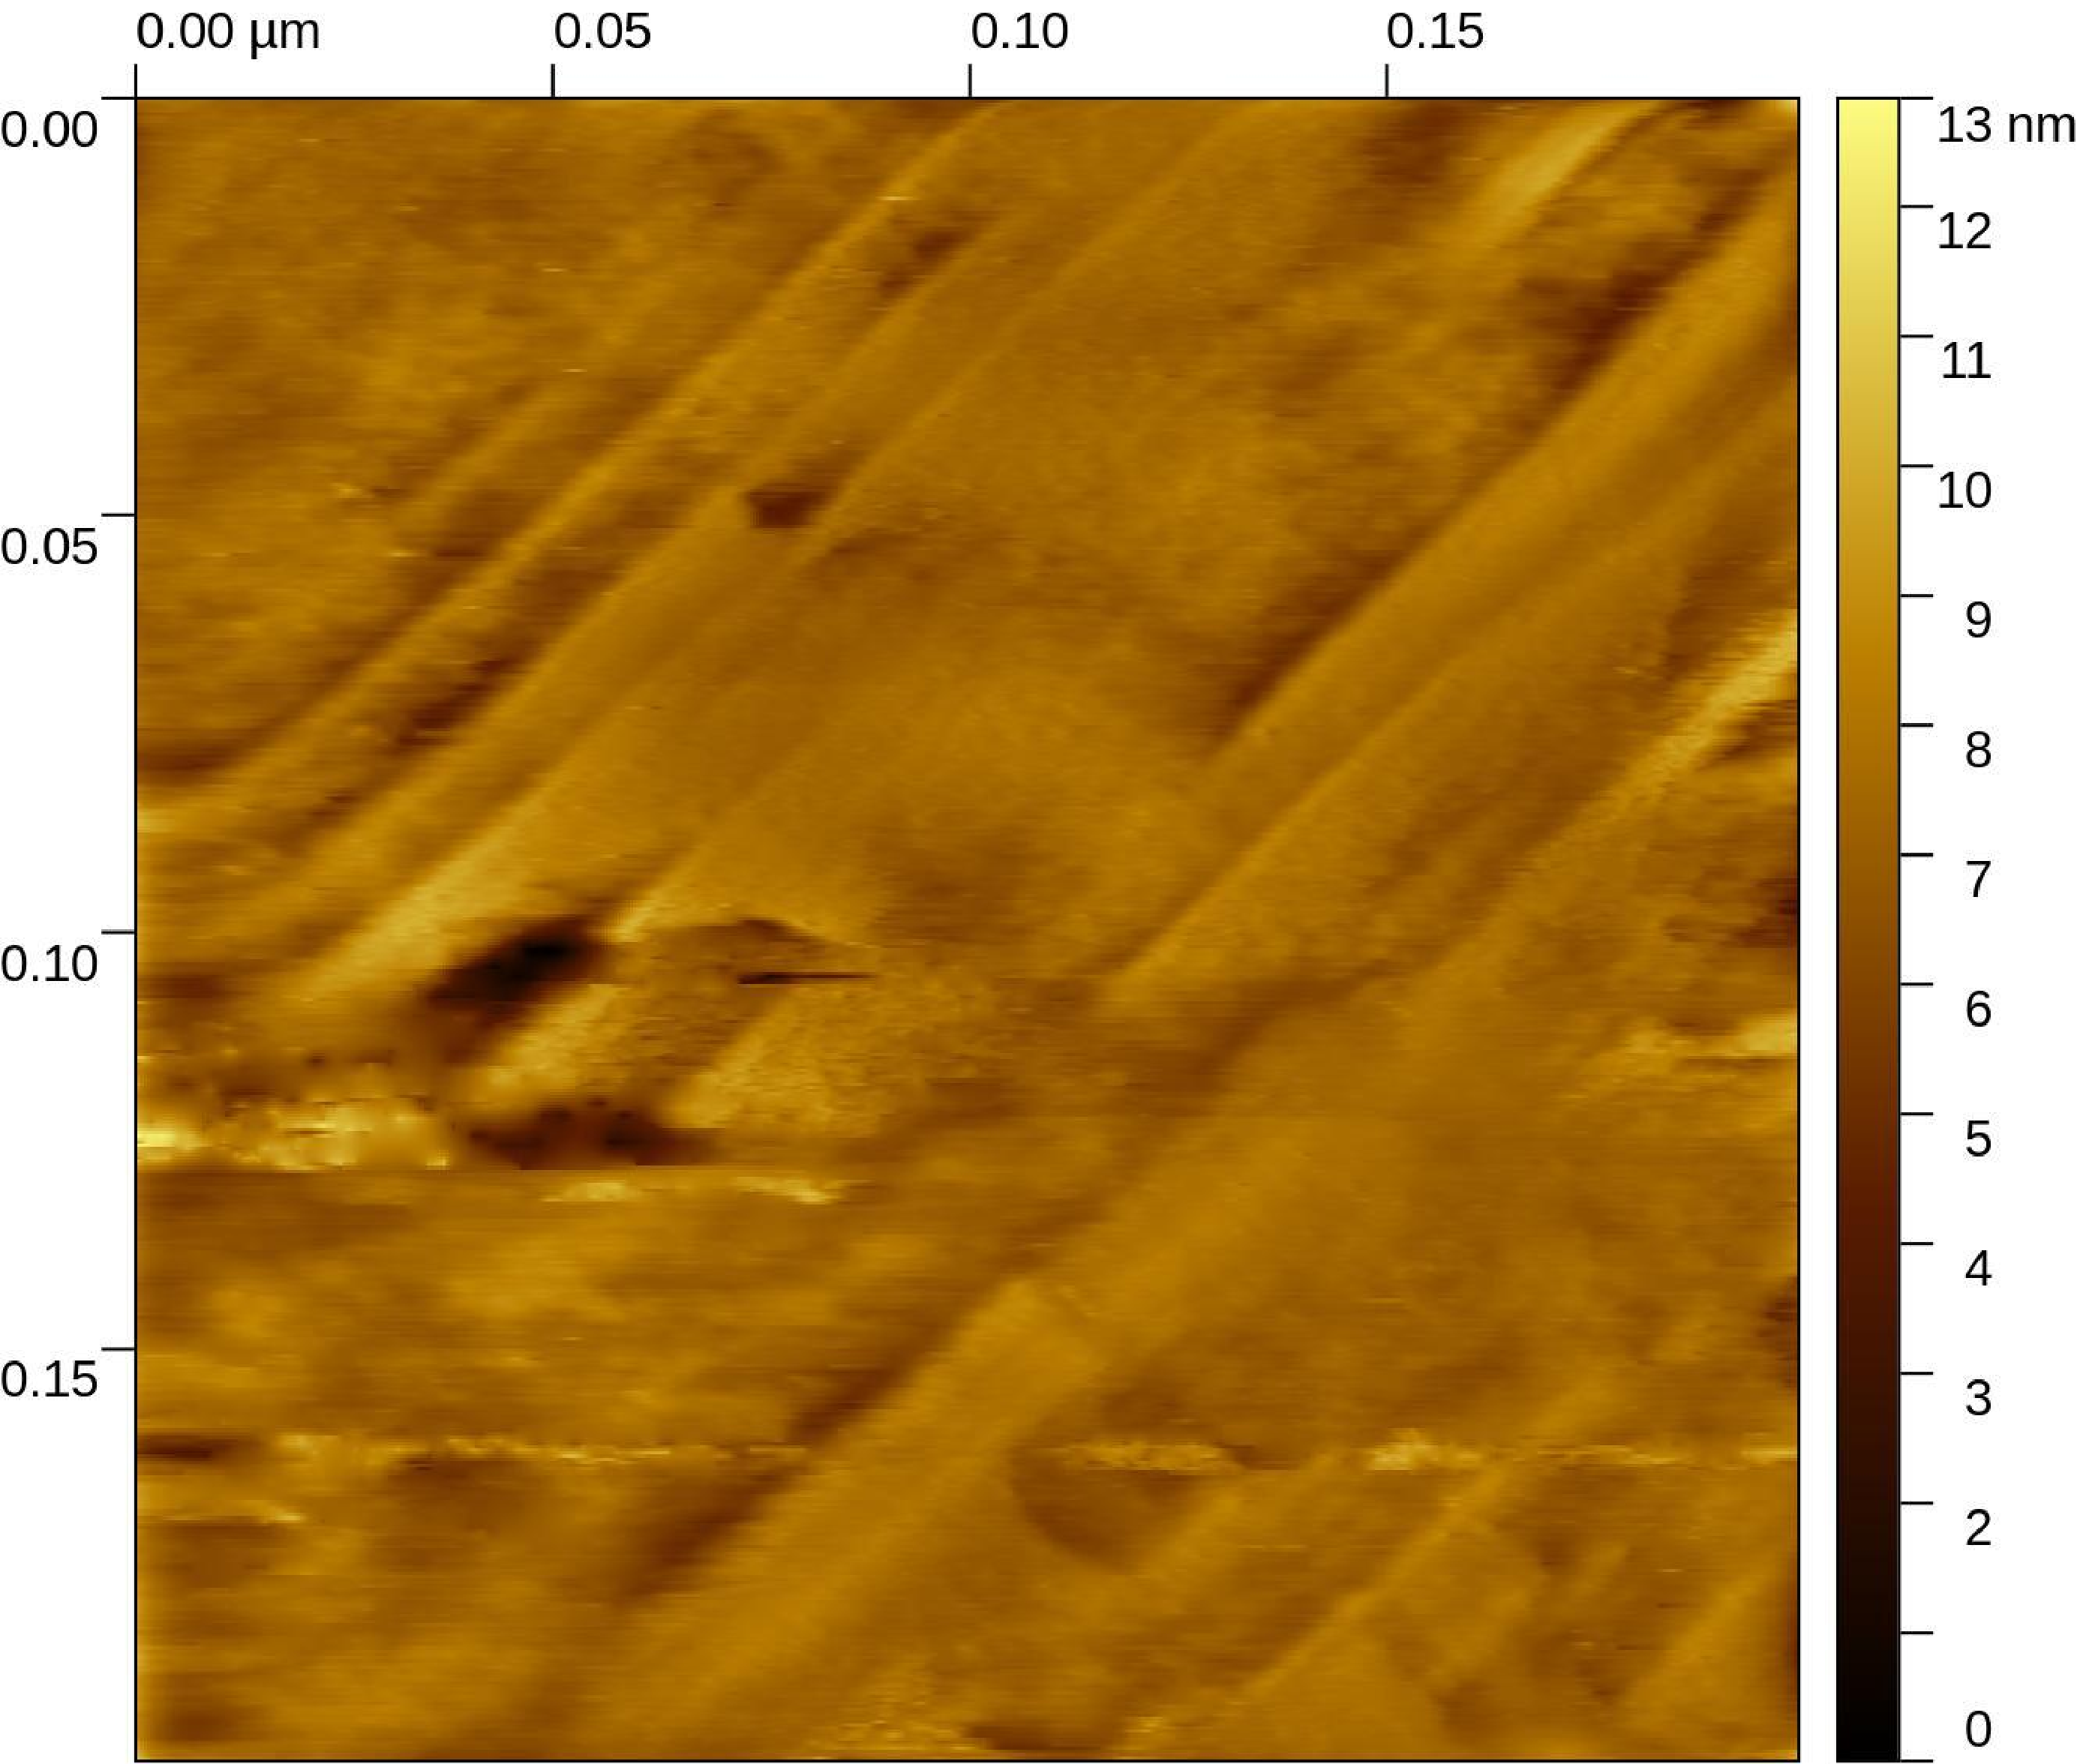
\includegraphics[width=0.7\textwidth]{../media/B2.5/Gold.pdf}
	\caption{Terrassen, Quelle: \cite{Grover}, \\
			Bias-Spannung $423.66 \mathrm{\,mV}$, Strom $3.5 \mathrm{\,nA}$}
	\label{abb:Gold terassen}
\end{figure}

\newpage
\hypertarget{vergleich}{%
\subsubsection{Vergleich}\label{vergleich}}

Die von uns erstellten Messungen unterscheiden sich massiv von den bereitgestellten Messungen. Alle Messungen haben eine vergleichbare Bias--Spannung, die Stromstärken unterscheiden sich jedoch.

Insbesondere die bereitgestellte Messung der Stufenkante (Abb. \ref{abb:Gold Stufenkante}) ist bei einer deutlich geringeren Stromstärke als alle anderen Messungen an Gold vorgenommen worden, die Stromstärken unterscheiden sich um einen Faktor $6$ von unseren Stromstärken. Die Stromstärken von unseren Messungen sind jedoch auch um ca. $30\%$ größer als die bereitgestellte Messung der Terassen (Abb. \ref{abb:Gold terassen}) bei $3.5 \mathrm{\,nA}$.

Dies unterstützt die These, dass unsere Probe nicht sauber ist und eine Barriere aus Fremdstoffen die Tunnelwahrscheinlichkeit verringert.

\hypertarget{austrittsarbeit-1}{%
\subsubsection{Austrittsarbeit}\label{austrittsarbeit-1}}

Die Austrittsarbeit $\phi$ ist die Differenz zwischen Potentialbarriere $V_0$ und der Energie $E$ der tunnelnden Elektronen. Mithilfe der Relationen für die Tunnelwahrscheinlichkeit \eqref{eq:Tunnelwkt Kappa} und den Tunnelstrom \eqref{eq:Tunnelstrom} kann man die Austrittsarbeit ermitteln. Hierzu wird eine Proportionalitätskonstante $c$ eingeführt.

\begin{figure}[ht]
	\centering
	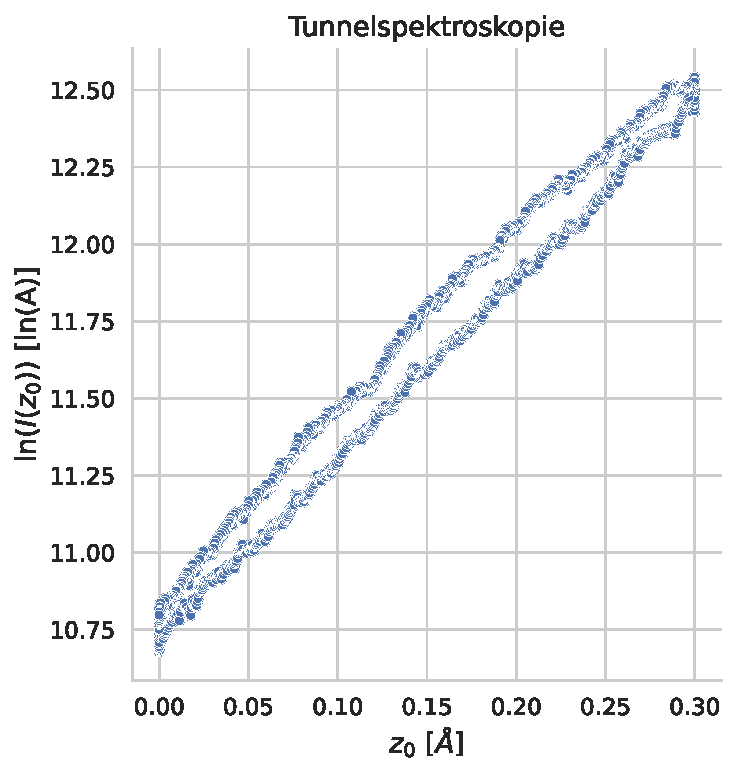
\includegraphics[width=0.5\textwidth]{../media/B2.5/Spektroskopie_2.pdf}
	\caption{Spektroskopiemessung, aufgetragen ist $\ln{I(z)}$ gegen $z$}
	\label{abb:Spektroskopie}
\end{figure}

\begin{eqnarray}
    I(z) &=& c \cdot \exp\left[-2\frac{\sqrt{2m_e\cdot \phi}}{\hbar} z\right] \\
    \ln I(z)
        &=& \ln(c)
            + \left(-2\frac{\sqrt{2m_e}}{\hbar}\right)
            \cdot \sqrt{\phi} \cdot z \\
    \ln I(z) &=& \ln(c) + 0.51 \mathrm{\,\frac{\sqrt{eV}}{\mathrm{\mathring{A}}}}\cdot \sqrt{\phi} \cdot z \label{eq: ln(Tunnelstrom)}
\end{eqnarray}

\noindent
Im letzten Schritt wurden die Naturkonstanten passend eingesetzt.
\cite{Anleitung} Dadurch kann die Austrittsarbeit aus der Steigung $m$ einer
Regression von $\ln I(z)$ ermittelt werden.
\begin{eqnarray}
    \phi &=& \left(\frac{m}{0.51}\right)^2 \mathrm{\,\frac{\AA^2}{eV}} \label{eq:Austrittsarbeit}
\end{eqnarray}

\noindent
Dadurch kann $\phi$ in der Einheit $\mathrm{eV}$ aus der Steigung $m$ in $\mathrm{\AA^{-1}}$ ermittelt werden, wie es in Gleichung \eqref{eq:Austrittsarbeit} beschrieben ist. Es ergeben sich folgende Ergebnisse, von denen die erste Hälfte aus der ersten und die zweite Hälfte aus der zweiten Messung stammen. Ein Messergebnis ist repräsentativ für alle in Abbildung \ref{abb:Spektroskopie} dargestellt.

\begin{table}[h!]
	\centering
	\begin{tabular}{cc}
		Steigung $m$ in $\mathrm{\mathring A}^{-1}$
			& $\phi$ in $\mathrm{eV}$ \\
		\hline
		$4.40 \pm 0.02$ & \ $74.283 \pm 0.002$ \\
		$6.91 \pm 0.03$ & $183.471 \pm 0.004$ \\
		$6.86 \pm 0.03$ & $180.925 \pm 0.004$ \\
		$6.49 \pm 0.03$ & $161.996 \pm 0.003$ \\
		$7.16 \pm 0.02$ & $196.918 \pm 0.002$ \\
		$5.18 \pm 0.02$ & $103.284 \pm 0.002$ \\
		$4.22 \pm 0.02$ & \ $68.402 \pm 0.001$ \\
		$5.59 \pm 0.02$ & $120.152 \pm 0.001$ \\
		$5.81 \pm 0.02$ & $129.797 \pm 0.001$ \\
		$5.64 \pm 0.02$ & $122.115 \pm 0.002$ \\
	\end{tabular}
	\caption{Steigung $m$ und Austrittsarbeit $\phi$\\
		nach Gleichungen \eqref{eq: ln(Tunnelstrom)} und \eqref{eq:Austrittsarbeit}}
	\label{table:Austrittsarbeit}
\end{table}

Die ermittelten Austrittsarbeiten $\phi$ sind sehr viel größer als erwartet, Literaturwerte sind in der Größenordnung von $5.3\mathrm{\,eV} - 5.45\mathrm{\,eV}$ \cite{Sachtler} oder um die $4\mathrm{\,eV}$ \cite{Anleitung} zu finden. Unsere Messwerte weichen um einen Faktor von ca. $17$ bis $50$ davon ab.

Dies bedeutet, dass die gemessene Austrittsarbeit extrem viel höher ist als theoretisch der Fall sein sollte. Dies könnte mit Fremdmaterial auf der Probe erklärt werden. Dieses erhöht die Potentialbarriere immens, wodurch sehr viel höhere Energien notwendig sind, um das Tunneln von Elektronen zu ermöglichen.

\hypertarget{graphit-hopg}{%
\subsection{Graphit (HOPG)}\label{graphit-hopg}}
Unsere eigenen Messungen in diesem Abschnitt waren sehr schlecht. Wie auch die Goldprobe ist diese Probe sehr wahrscheinlich verschmutzt, weiterhin waren auch hier Kratzer mit dem bloßen Auge sichtbar.

In Abbildung \ref{abb:hocp own: Fremdkörper} sieht man links einen Fremdkörper, rechts könnte es sich um Schäden oder einen weiteren Fremdkörper handeln.

In Abbildung \ref{abb:hocp own: atomar} sollten Atome gemessen werden, dies ist allerdings nicht erfolgreich gewesen. Die Ergebnisse sollten wie die in den Abbildungen \ref{fig:hopg_1} oder \ref{fig:hopg_2} aussehen. Hier könnte es sein, dass ein schlecht leitendes Material, z.B. eine Fettschicht, auf der Probe war, die die Messergebnisse verschlechtert hat.

Weiterhin sind die Höhenunterschiede innerhalb der Messungen in allen Fällen extrem groß. Um eine sinnvolle Auswertung durchführen zu können wurden uns andere Messergebnisse zur Verfügung gestellt. \cite{Grover}

Im Vergleich der Bias--Spannungen fällt auf, dass unsere Spannungen sehr viel größer sind als bei den zur Verfügung gestellten Daten. Insbesondere bei dem Versuch, Atome zu messen, ist dieser Unterschied mit einem Faktor von ca. $15$ extrem groß. Dies spricht für z.B. Fremdmaterial, das eine exakte Messung stört.

\begin{figure}[h!]
	\begin{minipage}{\textwidth}
		\begin{minipage}[T]{0.5\textwidth}
			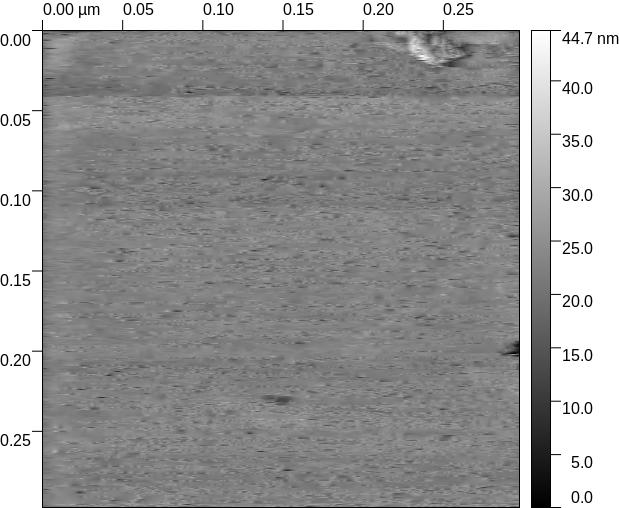
\includegraphics[width=\textwidth]{../media/B2.5/Graphit_3.jpg}
			\caption{Bias-Spannung $961.86 \mathrm{\,mV}$,
				Strom $6.3 \mathrm{\,nA}$}
		\end{minipage}
		\begin{minipage}[T]{0.5\textwidth}
			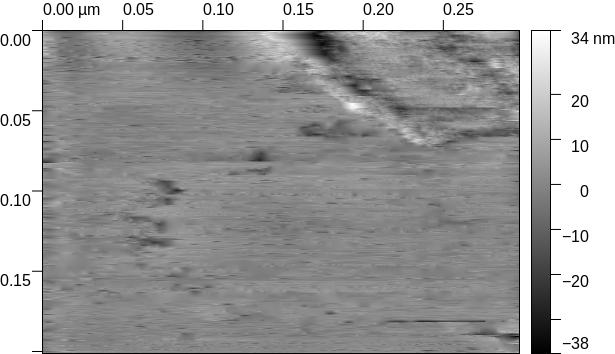
\includegraphics[width=\textwidth]{../media/B2.5/Graphit_1.jpg}
			\caption{Bias-Spannung $961.86 \mathrm{\,mV}$,
				Strom $6.3 \mathrm{\,nA}$}
		\end{minipage}
		\caption{Fremdkörper (links) und Schäden (rechts) in HOCP}
		\label{abb:hocp own: Fremdkörper}
	\end{minipage}
	\begin{minipage}{\textwidth}
		\begin{minipage}[t]{0.5\textwidth}
			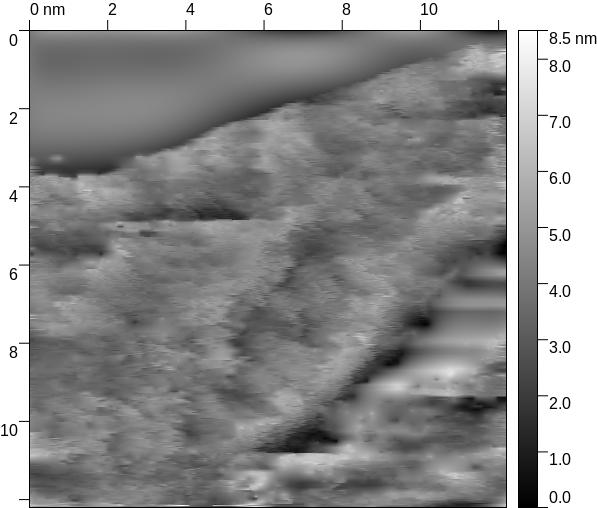
\includegraphics[width=\textwidth]{../media/B2.5/Graphit_2.jpg}
			\caption{Bias-Spannung $867.90 \mathrm{\,mV}$,
				Strom $5.9 \mathrm{\,nA}$}
		\end{minipage}
		\begin{minipage}[t]{0.5\textwidth}
			\centering
			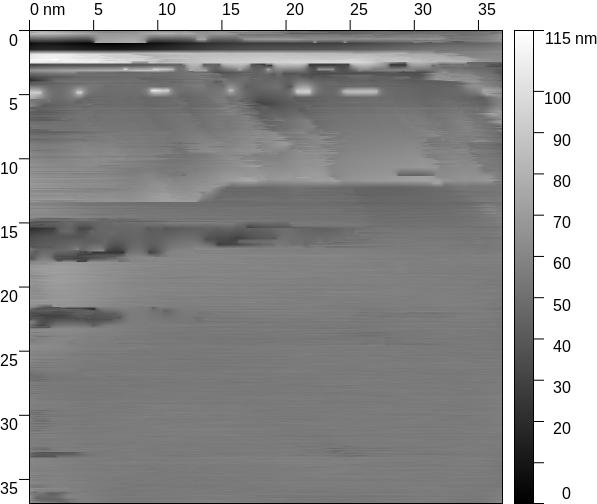
\includegraphics[width=\textwidth]{../media/B2.5/Graphit_4.jpg}
			\caption{Bias-Spannung $763.00 \mathrm{\,mV}$,
				Strom $6.3 \mathrm{\,nA}$}
		\end{minipage}
		\caption{HOCP in atomarer Auflösung - fehlerhafte Messungen}
		\label{abb:hocp own: atomar}
	\end{minipage}
\end{figure}


\hypertarget{messungen HOPG}{%
\subsubsection{Stufenkante}\label{messungen HOPG}}
In Abbildung \ref{abb:Stufenkante HOPG} ist eine Aufnahme von Graphit zu sehen. In ihr ist eine gerade Kante zu entdecken, die das Bild horizontal schneidet. Hierbei handelt es sich um eine Stufenkante.

Kurz oberhalb der Kante ist eine hellere Schicht zu entdecken, die eine erhöhte Region darstellt. Darauf folgt eine dunkle Linie, eine tief liegende Region. Der Höhenunterschied, der durch die Stufenkante hervorgerufen wird, ist daher deutlich zu erkennen. Da es oberhalb der Kante heller ist als unterhalb, verläuft die Stufe von oben nach unten betrachtet in die Bildebene hinein.

Eine interessante Beobachtung ist, dass nach einem dunkleren Teil nach der dunklen Linie die Region relativ schnell wieder eine ähnliche Tiefe annimmt, wie vor der ganzen Kante. Nach der Stufenkante wächst die Höhe der Region langsam wieder an, bis die ungefähre Höhe vor der Stufenkante erreicht ist.
%Ein dazu passendes Verhalten ist im nächsten Abschnitt in der Profildarstellung der Stufenkante zu sehen.

\begin{figure}[h!]
	\centering
	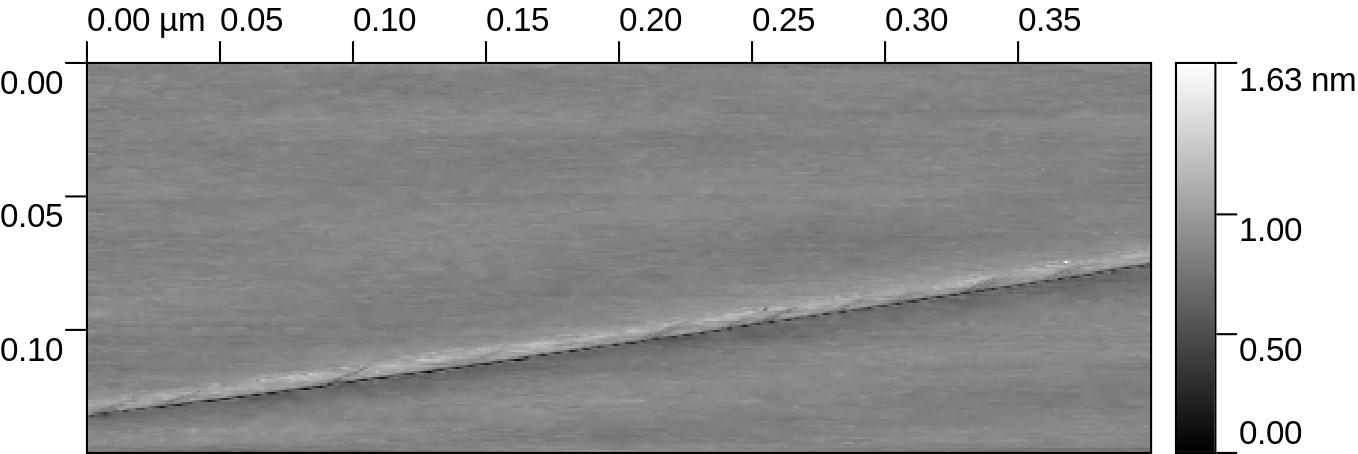
\includegraphics[width=0.7\textwidth]{../media/B2.5/HOPG Stufenkante.jpg}
	\caption{Stufenkante in Graphit, \\
		Bias-Spannung $449.74 \mathrm{\,mV}$,
		Strom $0.48 \mathrm{\,nA}$, \\
		Quelle \cite{Grover}}
	\label{abb:Stufenkante HOPG}
\end{figure}

\hypertarget{Stufenkante Höhe}{
\subsubsection{Höhe der Stufenkante}\label{Stufenkante Höhe}}
Um die Höhe der Stufenkante zu bestimmen, wurde in Gwyddion \cite{Gwyddion} ein Profil senkrecht zur Stufenkante gelegt. Das Ergebnis ist in Abbildung \ref{fig:stufenkante_profil} dargestellt. Die Höhe $h$ ergibt sich nun als die Differenz des Punktes vor der Kante $h_1$ und des Punktes nach der Kante $h_2$.

Der Fehler der Höhen $h_1$ und $h_2$ ist durch die Angabe in Gwyddion als $\Delta h_i = 0.0005 \,\AA$ angegeben. Der Fehler der Höhe der Stufenkante $h$ folgt durch Gaußsche Fehlerfortpflanzung.

\begin{eqnarray}
	h &=& h_1 - h_2 \\
	\Delta h &=& \sqrt{
			\left(\frac{\partial h}{\partial h_1} \Delta h_1\right)^2
			+ \left(\frac{\partial h}{\partial h_2} \Delta h_2\right)^2 } \\
			&=& \sqrt{(\Delta h_1)^2 + (-\Delta h_2)^2} \\
			&=& \sqrt{2} \Delta h_i \\
			&\approx& 0.0007 \,\AA \\
	\Rightarrow h &=& (4.5820 \pm 0.0007) \,\AA
\end{eqnarray}

\begin{figure}[h!]
	\centering
	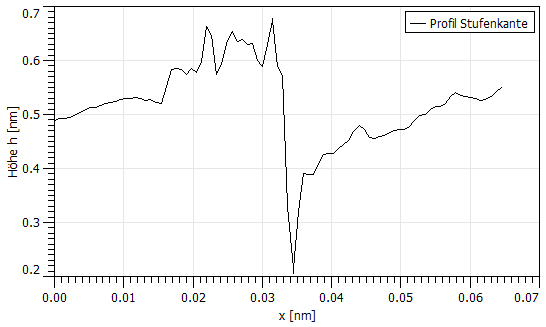
\includegraphics[width=0.7\textwidth]{../media/B2.5/HOPG_Stufenkante_Profil.png}
	\caption{Profil senkrecht zur Stufenkante}
	\label{fig:stufenkante_profil}
\end{figure}

Die Höhe der hier betrachteten Stufenkante beträgt also ca. $(4.5820 \pm 0.0007) \,\AA$. Der Literaturwert für den Abstand zweier Schichten in Graphit beträgt $3.35 \mathrm{\, \normalfont{\AA}}$. \cite{Anleitung} % S. 13

Unser Ergebnis ist mit ca. $4.5820 \mathrm{\, \normalfont{\AA}}$ deutlich größer, woran der Fehler unserer Messung nichts ändert. Dies lässt sich aber z.B. durch lokale Unebenheiten erklären, welche die Höhe der Stufenkante beeinflussen können. Weiterhin kann eine Ungenauigkeit in der Auflösung des Bildes zu Abweichungen in den Messwerten führen.

Unter diesen Berücksichtigungen sind wir dem Literaturwert mit unserem Ergebnis doch recht nah gekommen, sodass dieser Teil des Versuchs als Erfolg betrachtet werden kann.

\hypertarget{HOPC atomar}{
\subsubsection{Atomare Auflösung von Graphit}\label{HOPC atomar}}
In den Abbildungen \ref{fig:hopg_1} und \ref{fig:hopg_2} sind die atomaren Auflösungen von Graphit zu sehen, wobei die helleren Punkte die Atome repräsentieren. Dies ist durch den höheren Tunnelstrom an der Oberfläche der Atome begründet. \cite{Mizes}

Weiterhin kann die Form der einzelnen Atome und die Anordnung derer auf der resultierenden Abbildung durch eine asymmetrische Spitze verändert werden. \cite{Mizes} Es werden fünf verschiedene Abbildungsformen dargestellt, die auftreten können. Die Unterschiede sind durch unterschiedliche Spitzen begründet, nicht durch die Probe selbst.

Die linke atomare Abbildung \ref{fig:hopg_1} ist durch eine dreieckige Anordnung von Ellipsen dargestellt. Die rechte atomare Abbildung \ref{fig:hopg_2} ist dagegen eher eine Reihenanordnung von Ellipsen.

Es wurden daher keine verschiedenen Proben mit vermessen. Ledglich die Messspitze war bei den Messungen anders.

\begin{figure}[h!]
	\begin{minipage}[t]{0.5\textwidth}
		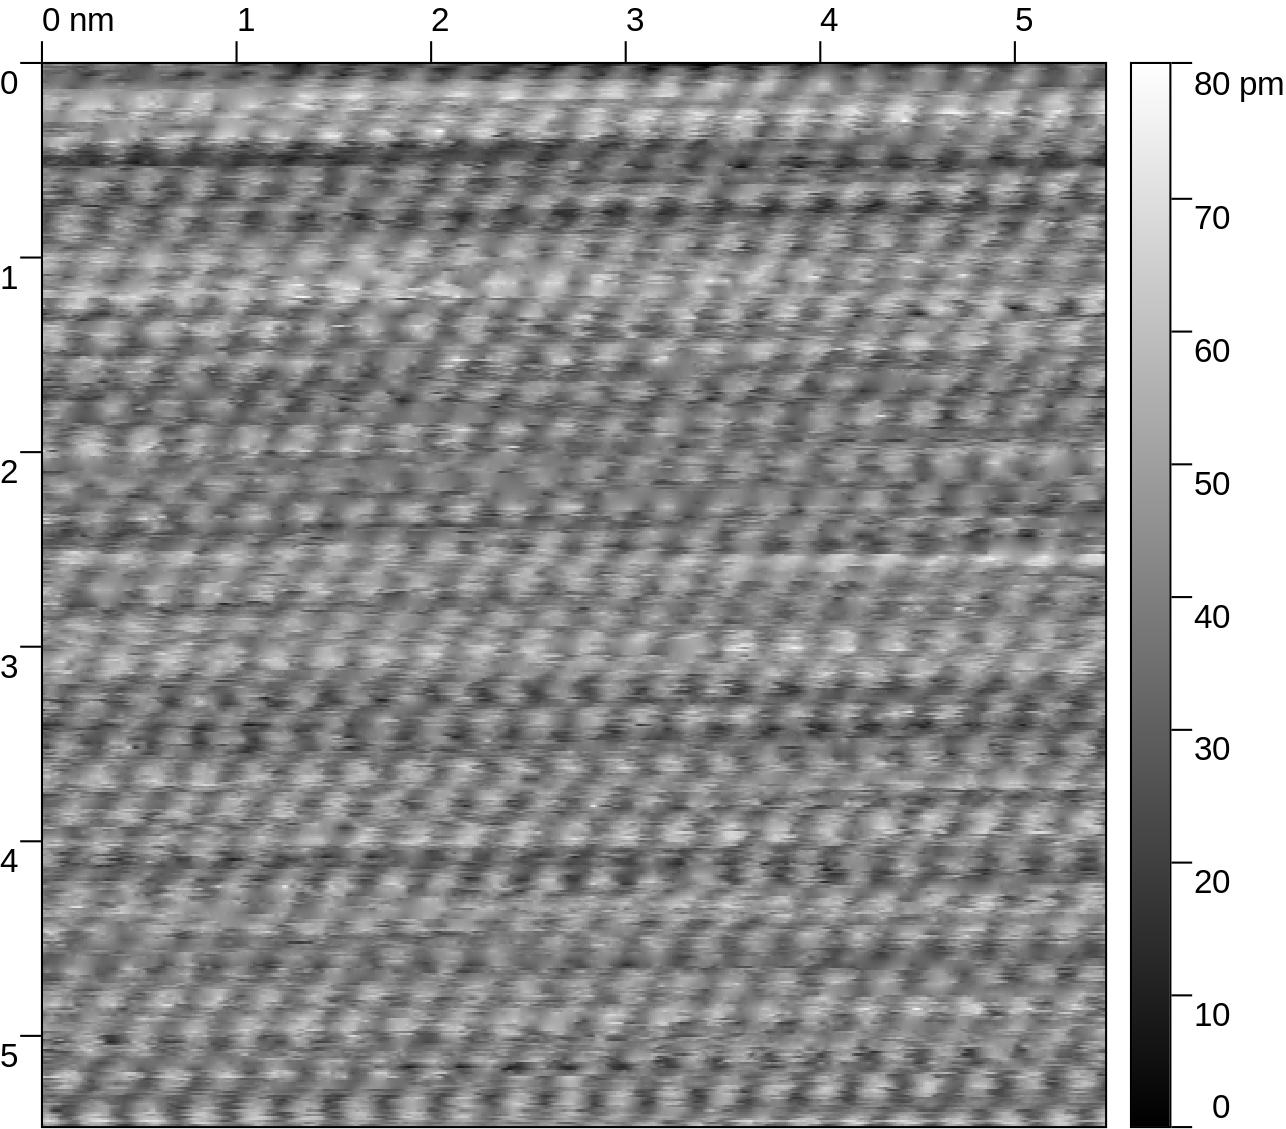
\includegraphics[width=\linewidth]{../media/B2.5/Atoms_1.jpg}
		\caption{dreieckige Anordnung, \\
			Bias-Spannung $49.82\mathrm{\,mV}$, Strom $1.7\mathrm{\,nA}$,
			\\Quelle \cite{Grover}}
		\label{fig:hopg_1}
	\end{minipage}
	\begin{minipage}[t]{0.5\textwidth}
		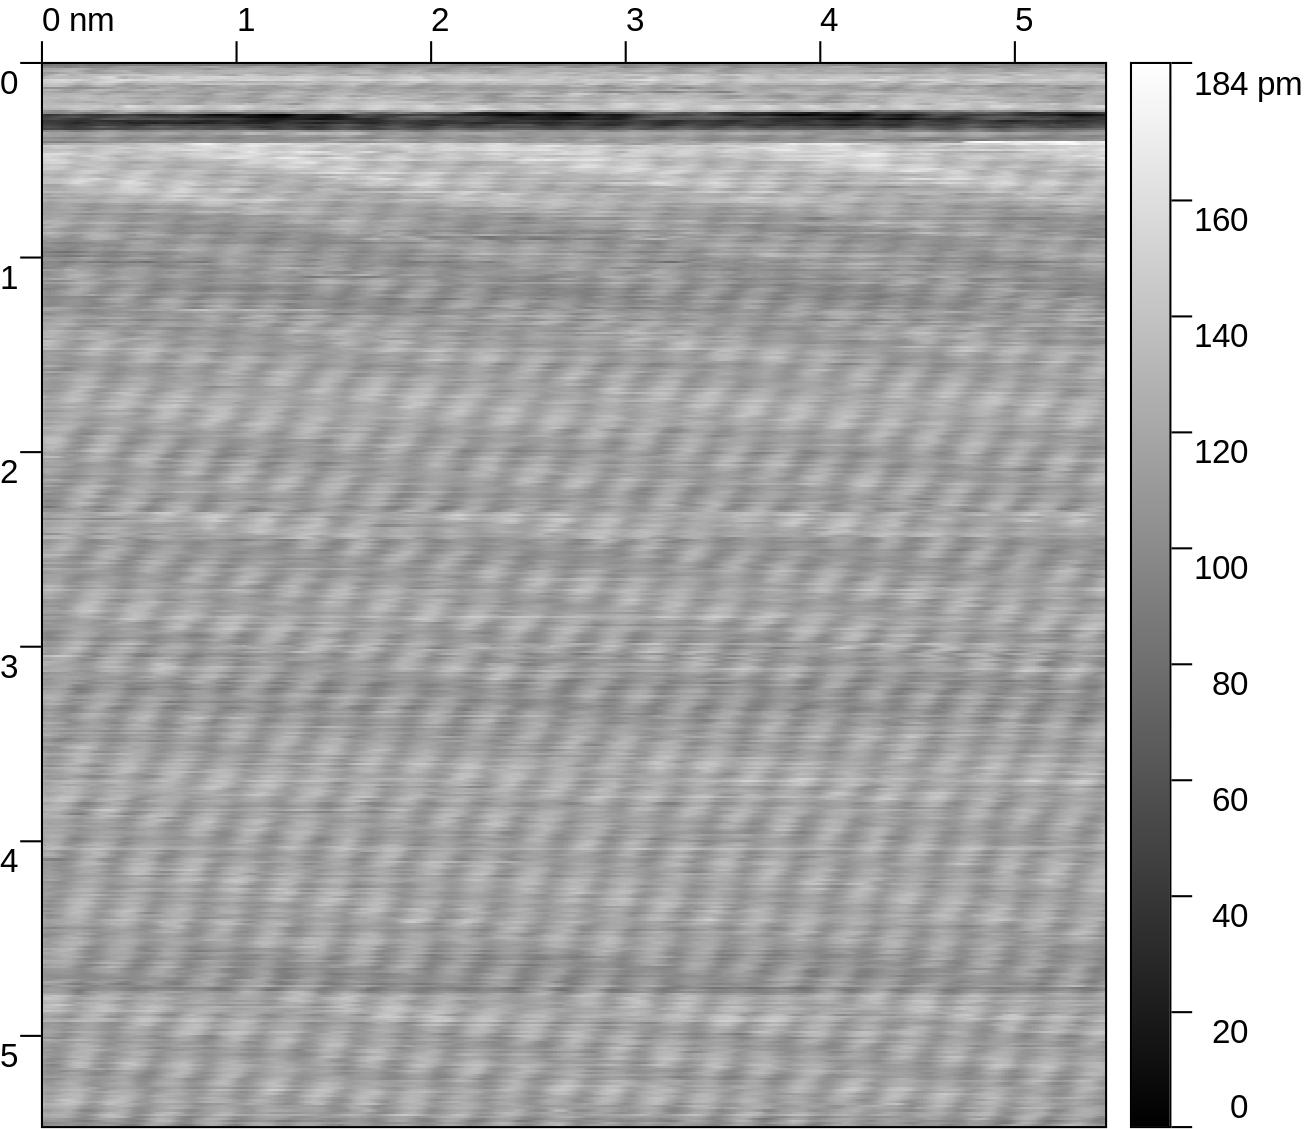
\includegraphics[width=\linewidth]{../media/B2.5/Atoms_2.jpg}
		\caption{Reihenanordnung,
			Bias-Spannung $40.90\mathrm{\,mV}$, Strom $8.6\mathrm{\,nA}$,
			\\Quelle \cite{Grover}}
		\label{fig:hopg_2}
	\end{minipage}
\end{figure}


\hypertarget{korrugation}{%
\subsubsection{Korrugation}\label{korrugation}}

Um die Korrugation von Graphit zu bestimmen, wird ein Profil über die Atome der drei dichtgepacktesten Richtungen auf die beiden Bilder gelegt. Daraus kann die jeweilige Korrugation als Differenz des Maximums und des Minimums der Amplituden bestimmt werden. Ein Mittelwert aus den drei Werten liefert die mittlere Korrugation von Graphit an der gemessenen Stelle, ihr Fehler wird durch die Mittlere Quadratsumme der Residuen (MQR) gebildet.

\begin{eqnarray}
	\bar{K} &=& \sum_{i=1}^n \frac{K_i}{n} \\
	\Delta \bar{K} &=& \sqrt{\frac{1}{n (n-1)} \cdot \sum_{i=1}^{n} (K_i -\bar{K})^2}
\end{eqnarray}

\noindent
Die drei dichtgepackten Richtungen der ersten atomaren Auflösung sind in Abbildung \ref{abb:hopg_with_profile_1} zu sehen. Mittels Gwyddion \cite{Gwyddion} lassen sich die Profile dieser Richtungen mit ihren minimalen und maximalen Amplituden anzeigen, siehe Abb. \ref{abb:hopg_profile_1}.

Die Ungenauigkeit liegt immer bei $\Delta A = \pm 0.001 \mathrm{\,nm}$. Die Korrugation der einzelnen Profile bestimmt sich nun aus dem Betrag der Differenz der minimalen und der maximalen Amplituden.

Analog wird die Korrugation aus der zweiten Messung bestimmt. In Abbildung \ref{abb:hopg_with_profile_2} sind die dichtestgepackten Richtungen zu sehen, die Profile sind in Abbildung \ref{abb:hopg_profile_2} dargestellt.

Alle Profile wurden entlang der Richtungen in den Abbildungen \ref{abb:hopg_with_profile_1} und \ref{abb:hopg_with_profile_2} von links nach rechts gemessen.

Die Ergebnisse der einzelnen Korrugationen sind in Tabelle \ref{table:Korrugation} dargestellt. Daraus ergeben sich folgende mittlere Korrugationen $\bar{K}$.

\begin{eqnarray}
	\bar{K_1} &=& 1.1 \mathrm{\,\mathring{A}} \pm 0.9 \mathrm{\,\mathring{A}} \\
	\bar{K_2} &=& 1.1 \mathrm{\,\mathring{A}} \pm 0.4 \mathrm{\,\mathring{A}}
\end{eqnarray}


\begin{table}[h!]
	\centering
	\begin{tabular}{lr|rrr|rrr}
		&& \multicolumn{3}{c}{Messung $1$} \vline& \multicolumn{3}{c}{Messung $2$} \\
		&& Profil $1$ & Profil $2$ & Profil $3$ & Profil $1$ & Profil $2$ & Profil $3$ \\
		\hline
		
		$A_\mathrm{min}$ &in $[\mathrm{nm}]$
			& $-41.01$ & $-40.93$ & $-40.87$
			& $-45.54$ & $-45.53$ & $-45.51$
			\\
		$A_\mathrm{max}$ &in $[\mathrm{nm}]$
			& $-40.83$ & $-40.81$ & $-40.84$
			& $-45.46$ & $-45.39$ & $-45.39$
			\\
		$K$  &in $[\mathrm{nm}]$
			& $0.18$ & $0.12$ & $0.03$
			& $0.08$ & $0.14$ & $0.12$
	\end{tabular}
	\caption{Korrugationsmessungen von HOPG}
	\label{table:Korrugation}
\end{table}

\begin{figure}[h!]
	\centering
	\begin{minipage}[t]{0.4\textwidth}
		\centering
		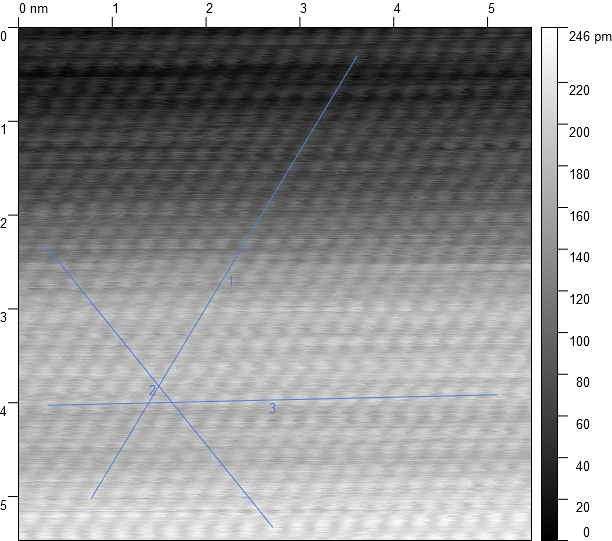
\includegraphics[width=\textwidth]{../media/B2.5/Atoms1_with_profileLines.png}
		\caption{Dichtgepackteste Richtungen der ersten atomaren Auflösung von Graphit\\
			Bias-Spannung $49.82\mathrm{\,mV}$, \\
			Strom $1.7\mathrm{\,nA}$}
		\label{abb:hopg_with_profile_1}
	\end{minipage}
	\begin{minipage}[t]{0.5\textwidth}
		\centering
		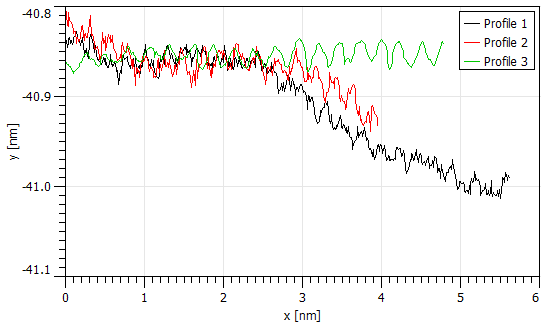
\includegraphics[width=\textwidth]{../media/B2.5/profilePlot_area1.png}
		\caption{Profile der drei dichtgepacktesten Richtungen der ersten atomaren Auflösung}
		\label{abb:hopg_profile_1}
	\end{minipage}
	\vspace{12pt}
	
	\begin{minipage}[t]{0.4\textwidth}
		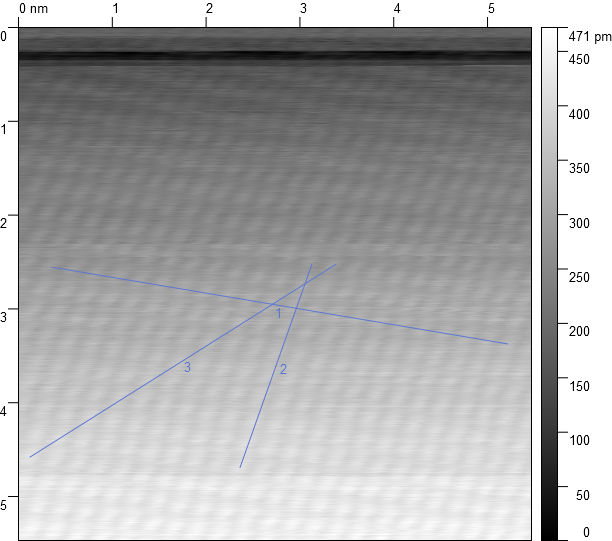
\includegraphics[width=\linewidth]{../media/B2.5/Atoms2_with_profileLines.png}
		\caption{Dichtgepackteste Richtungen der zweiten atomaren Auflösung von Graphit
			Bias-Spannung $40.90\mathrm{\,mV}$, \\
			Strom $8.6\mathrm{\,nA}$}
		\label{abb:hopg_with_profile_2}
	\end{minipage}
	\begin{minipage}[t]{0.5\textwidth}
		\centering
		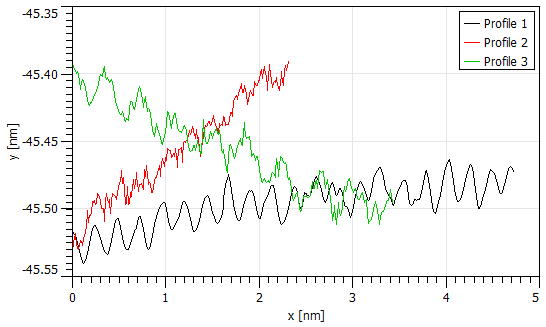
\includegraphics[width=\linewidth]{../media/B2.5/profilePlot_area2.png}
		\caption{Profile der drei dichtgepacktesten Richtungen der zweiten atomaren Auflösung}
		\label{abb:hopg_profile_2}
	\end{minipage}
\end{figure}

\clearpage
\hypertarget{fazit}{%
\section{Fazit}\label{fazit}}
Insgesamt ist die Arbeit mit dem STM ein interessanter Versuch. Dies wird jedoch massiv dadurch geschmähert, dass die Proben offensichtlich verunreinigt sind.

Diese These wird durch die hohe Austrittsarbeit in Gold, sowie durch die hohen Bias--Spannungen bei HOCP bestätigt. Ebenso wird sie durch die Messung von Fremdkörpern unterstützt. Dies ist ein interessantes Ergebnis, das noch einmal in der untenstehenden Abbildung dargestellt ist.

\begin{figure}[h!]
	\centering
	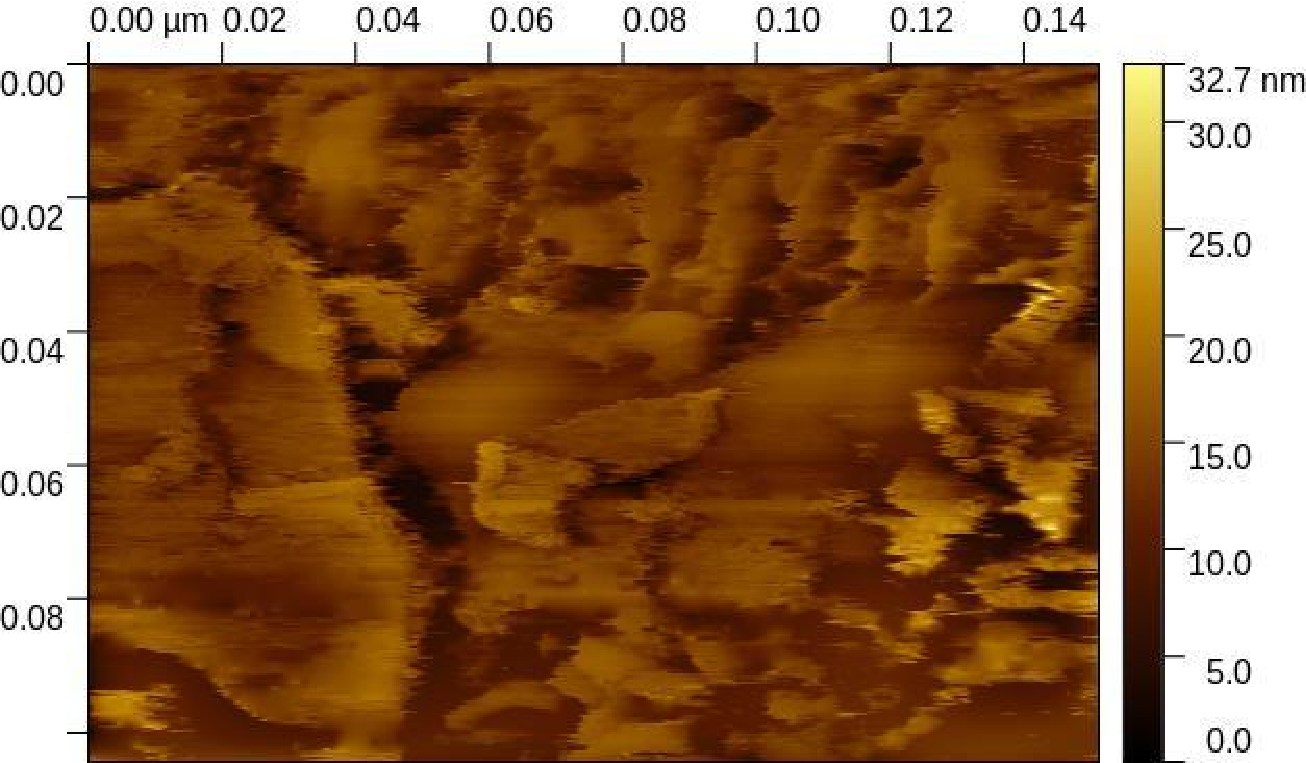
\includegraphics[width=0.7\textwidth]{../media/B2.5/Gold_gross.pdf}
\end{figure}

\noindent
Vermutlich spielt das Alter der Proben eine Rolle. Uns wurde mitgeteilt, dass schon von anderen versucht wurde, die Proben ordentlich zu reinigen, was aber wenig erfolgreich gewesen sei. Dies spricht dafür, dass die Proben für diesen Versuch nicht (mehr) geeignet sind.

Das ein guter Teil der Auswertung an Ergebnissen von fremden Messungen durchgeführt werden musste, ist schade. Man kann es als Erfahrung verbuchen, denn auch in anderen Situationen werden Daten ausgewertet, die nicht selbst gemessen wurden.

\clearpage
\hypertarget{literatur}{%
\section{Literaturverzeichnis}\label{literatur}}
\renewcommand{\section}[2]{} % remove extra title
\begin{thebibliography}{9}
\bibitem{Gwyddion}
	Gwyddion, \url{http://gwyddion.net}

\bibitem{WSxM}
	I. Horcas, R. Fernandez, J.M. Gomez-Rodriguez, J. Colchero, J. Gomez-Herrero and A. M. Baro, Rev.~Sci. Instrum. 78, 013705 (2007), \url{http://www.wsxm.eu}

\bibitem{Anleitung}
	Universität zu Köln, ``Versuch B.2.5. Rastertunnelmikroskopie'', März 2017, 	\url{https://ph2.uni-koeln.de/fileadmin/Lehre/PraktikumB/B2.5_Anleitung_2017_03.pdf}

\bibitem{Mizes}
	H. A. Mizes, W. A. Harrison und S.-i. Park, ``Multiple-tip interpretation of anomalous scanning-tunneling-microscopy images of layered materials'', Physical Review~B Volume~36, pp.~4491 - 4494, 15. September 1987

\bibitem{Gross}
	R. Gross und A. Marx, ``Festkörperphysik'', Oldenbourg Verlag, 2012

\bibitem{Sachtler}
	W. Sachtler, G. Dorgelo, A. Holscher, ``The work function of gold'', Science Direct, 1966,
	\url{https://doi.org/10.1016/0039-6028(66)90083-5}

\bibitem{Grover}
	Versuchsbetreuung: M.~Sc.~Catherine~Grover, Studentin der Festkörperphysik im PhD an der Universität zu Köln, \url{https://ph2.uni-koeln.de/en/research-groups/group-michely/members}

\bibitem{WikipediaTunneleffekt}
	Wikipedia, 31. Oktober 2010, \url{https://commons.wikimedia.org/wiki/File:TunnelEffektKling1.png}

\bibitem{WikipediaBravaisgitter}
	Wikipedia, 4. März 2022, \url{https://commons.wikimedia.org/wiki/File:Rectangular_unit_cells_centered.svg}

\bibitem{WikipediaGraphit}
	Wikipedia, 21. Oktober 2010, \url{https://commons.wikimedia.org/wiki/File:Graphit_gitter4.svg}

\bibitem{WikipediaFcc}
	Wikipedia, 06. Februar 2009, \url{https://commons.wikimedia.org/wiki/File:Cubic,_face-centered.png}

\bibitem{USDoE}
	U.S. Department of Energy, ``Material Science. DOE Fundamentals Handbook, Volume 1 and 2'', January 1993, \url{https://www.standards.doe.gov/standards-documents/1000/1017-BHdbk-1993-v1/@@images/file}

\bibitem{WikipediaStufe}
	Wikipedia, 22. Januar 2011, \url{https://de.wikipedia.org/wiki/Datei:Dislocation_edge_d2.svg}

\bibitem{WikipediaSchraube}
	Wikipedia, 27. Januar 2011, \url{https://de.wikipedia.org/wiki/Datei:Dislocation_screw_e.svg}

\end{thebibliography}

\end{document}
